\section{数据探索}
\label{sec:data_exploration}

\subsection{各维度可视化结果}
本研究的可视化分析基于原始表达值与缺失值填充后的数据，以呈现真实分布；
在聚类与分类建模前，会对特征执行标准化处理，以满足模型对特征尺度的要求。
\subsubsection{原始数据缺失值分布}
\begin{figure}[htbp]
    \centering
    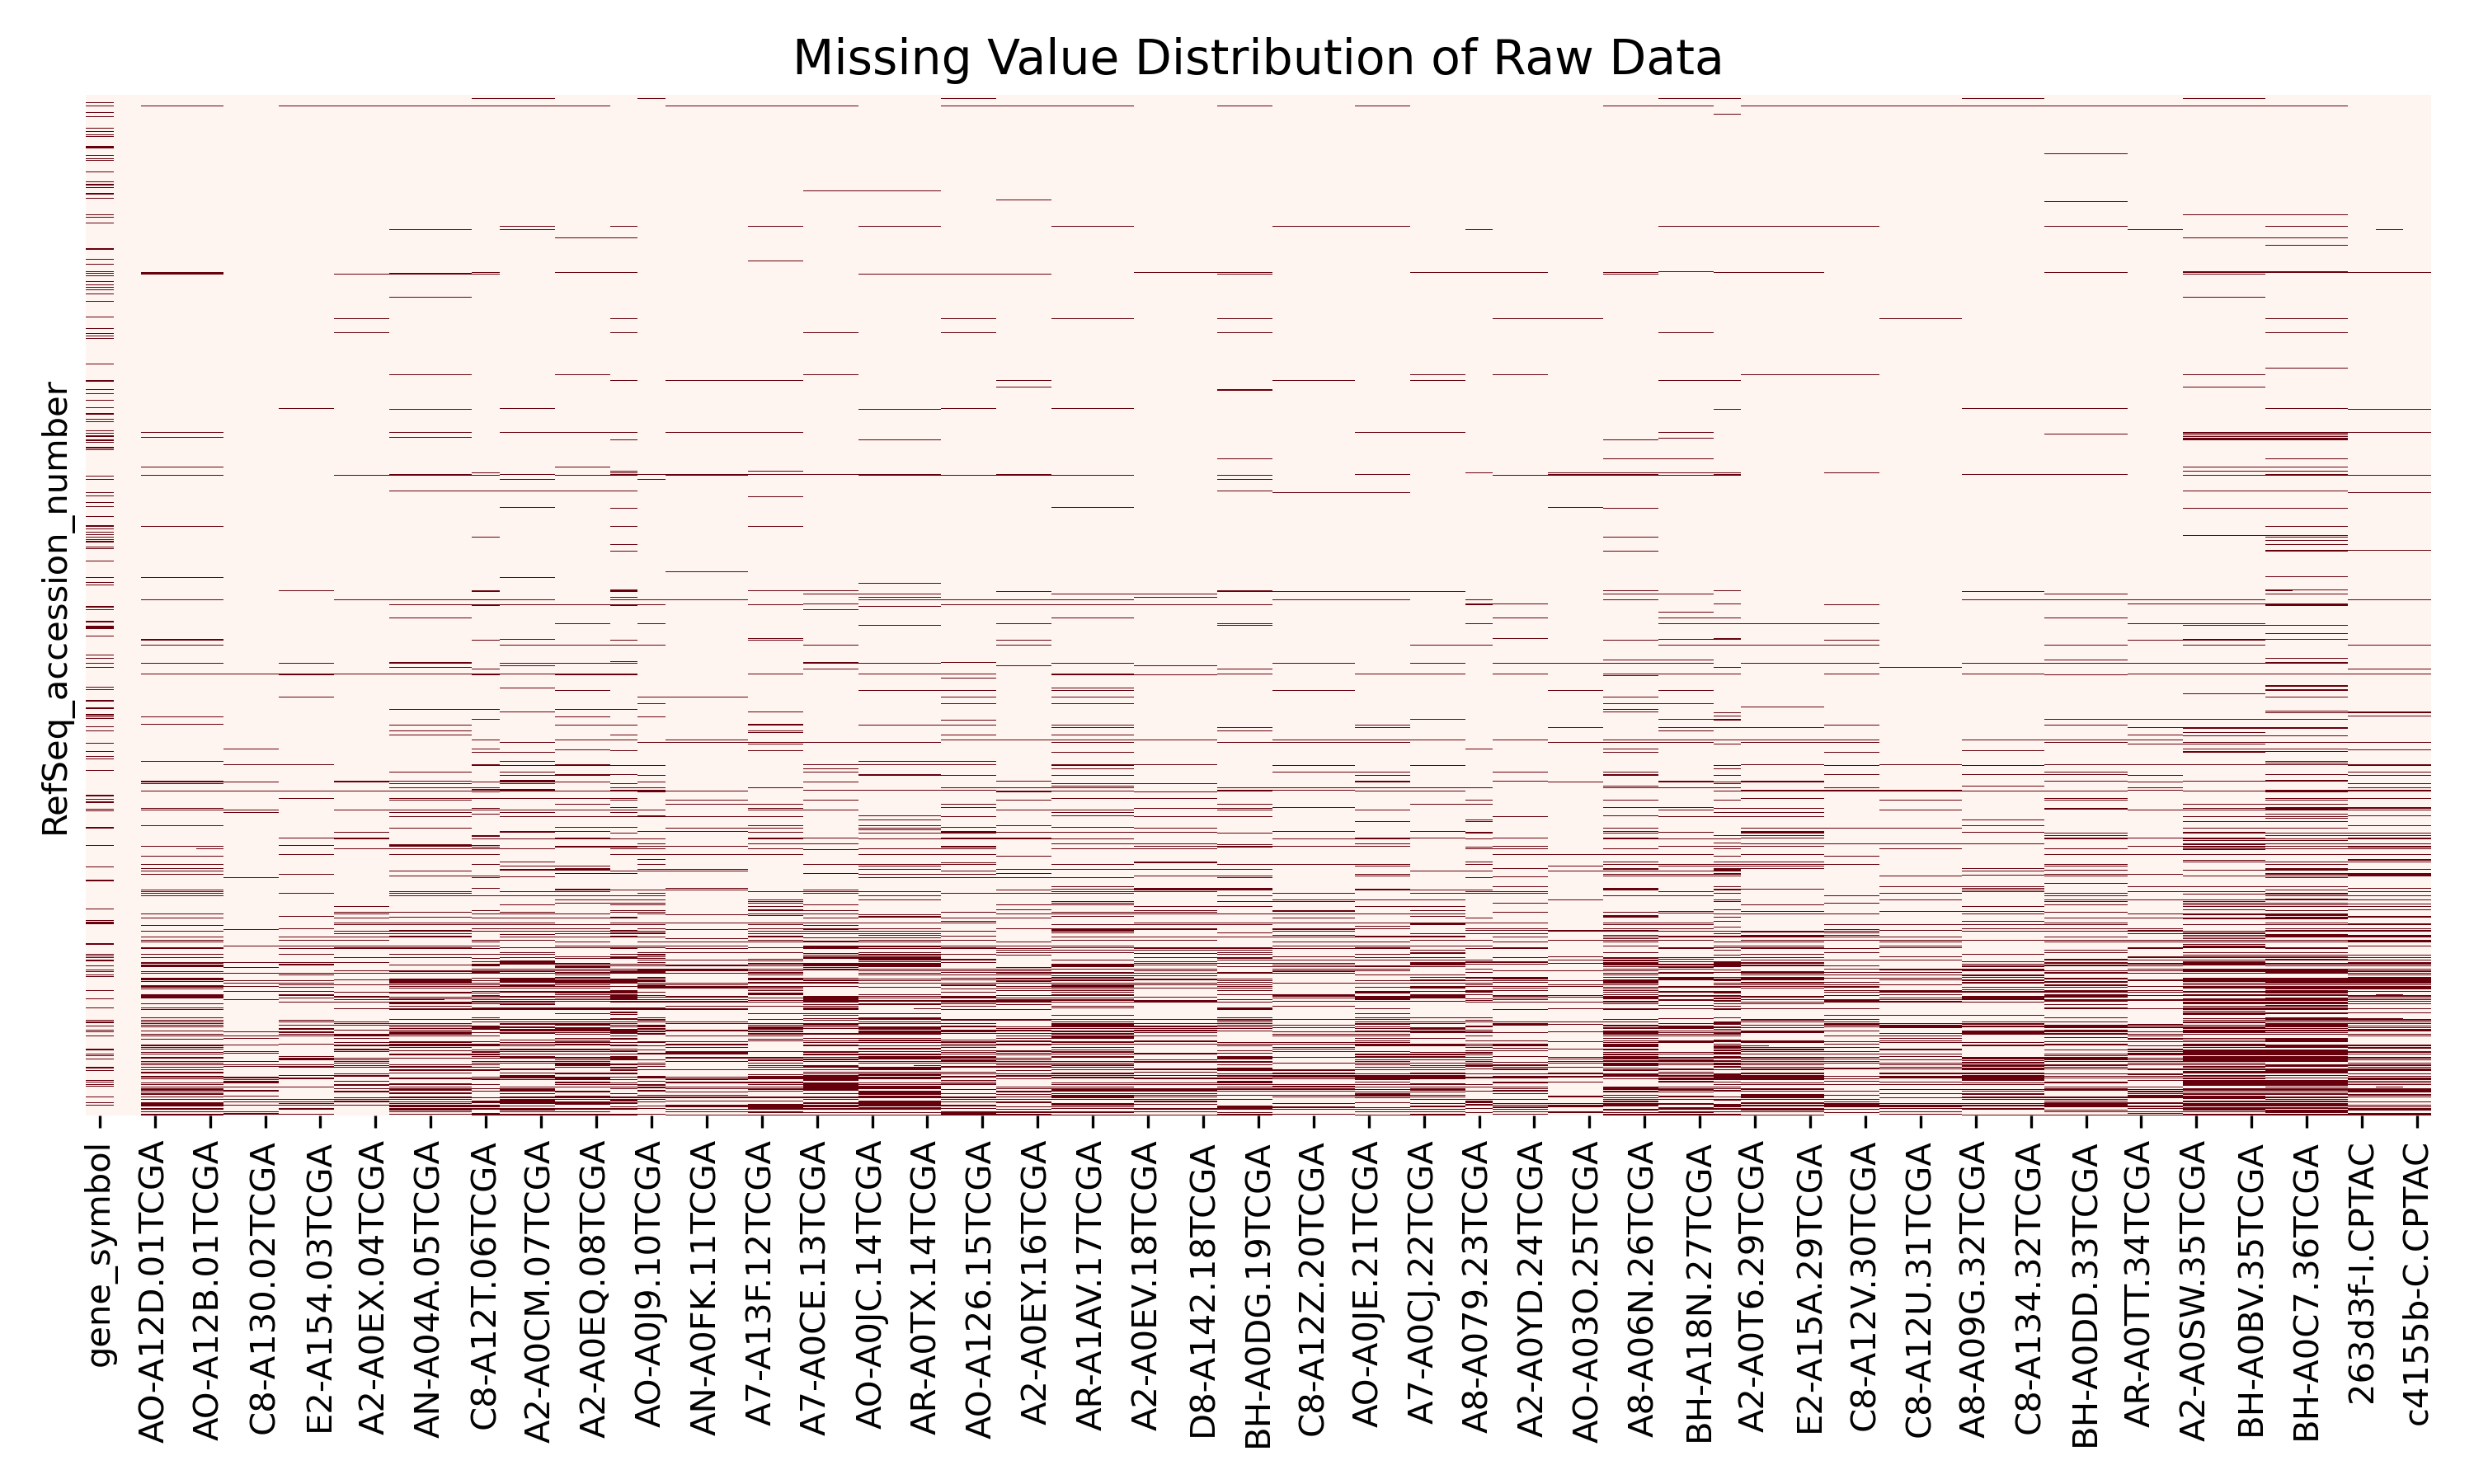
\includegraphics[width=0.85\textwidth]{./figures/data_preprocessing/1_missing_value.png}
    \caption{原始蛋白质数据缺失值分布热图}
    \label{fig:missing_value}
\end{figure}
在 77 个匹配癌症样本和 43 个可匹配 PAM50 蛋白特征中，共有 323 个缺失表达值，占全部
\(77\times 43=3311\) 个表达值的 9.76\%。整体上缺失值分布较分散，但不同蛋白之间缺失率并不完全一致；
例如 \texttt{NP\_002458} 与 \texttt{NP\_569082} 的缺失率分别约为 71.4\% 和 68.8\%。
因此，本研究采用中位数填充以保留样本量，同时在解释特征重要性时避免将高缺失蛋白过度解读为稳定生物标志物。

\subsubsection{原始蛋白质表达值分布}
\begin{figure}[htbp]
    \centering
    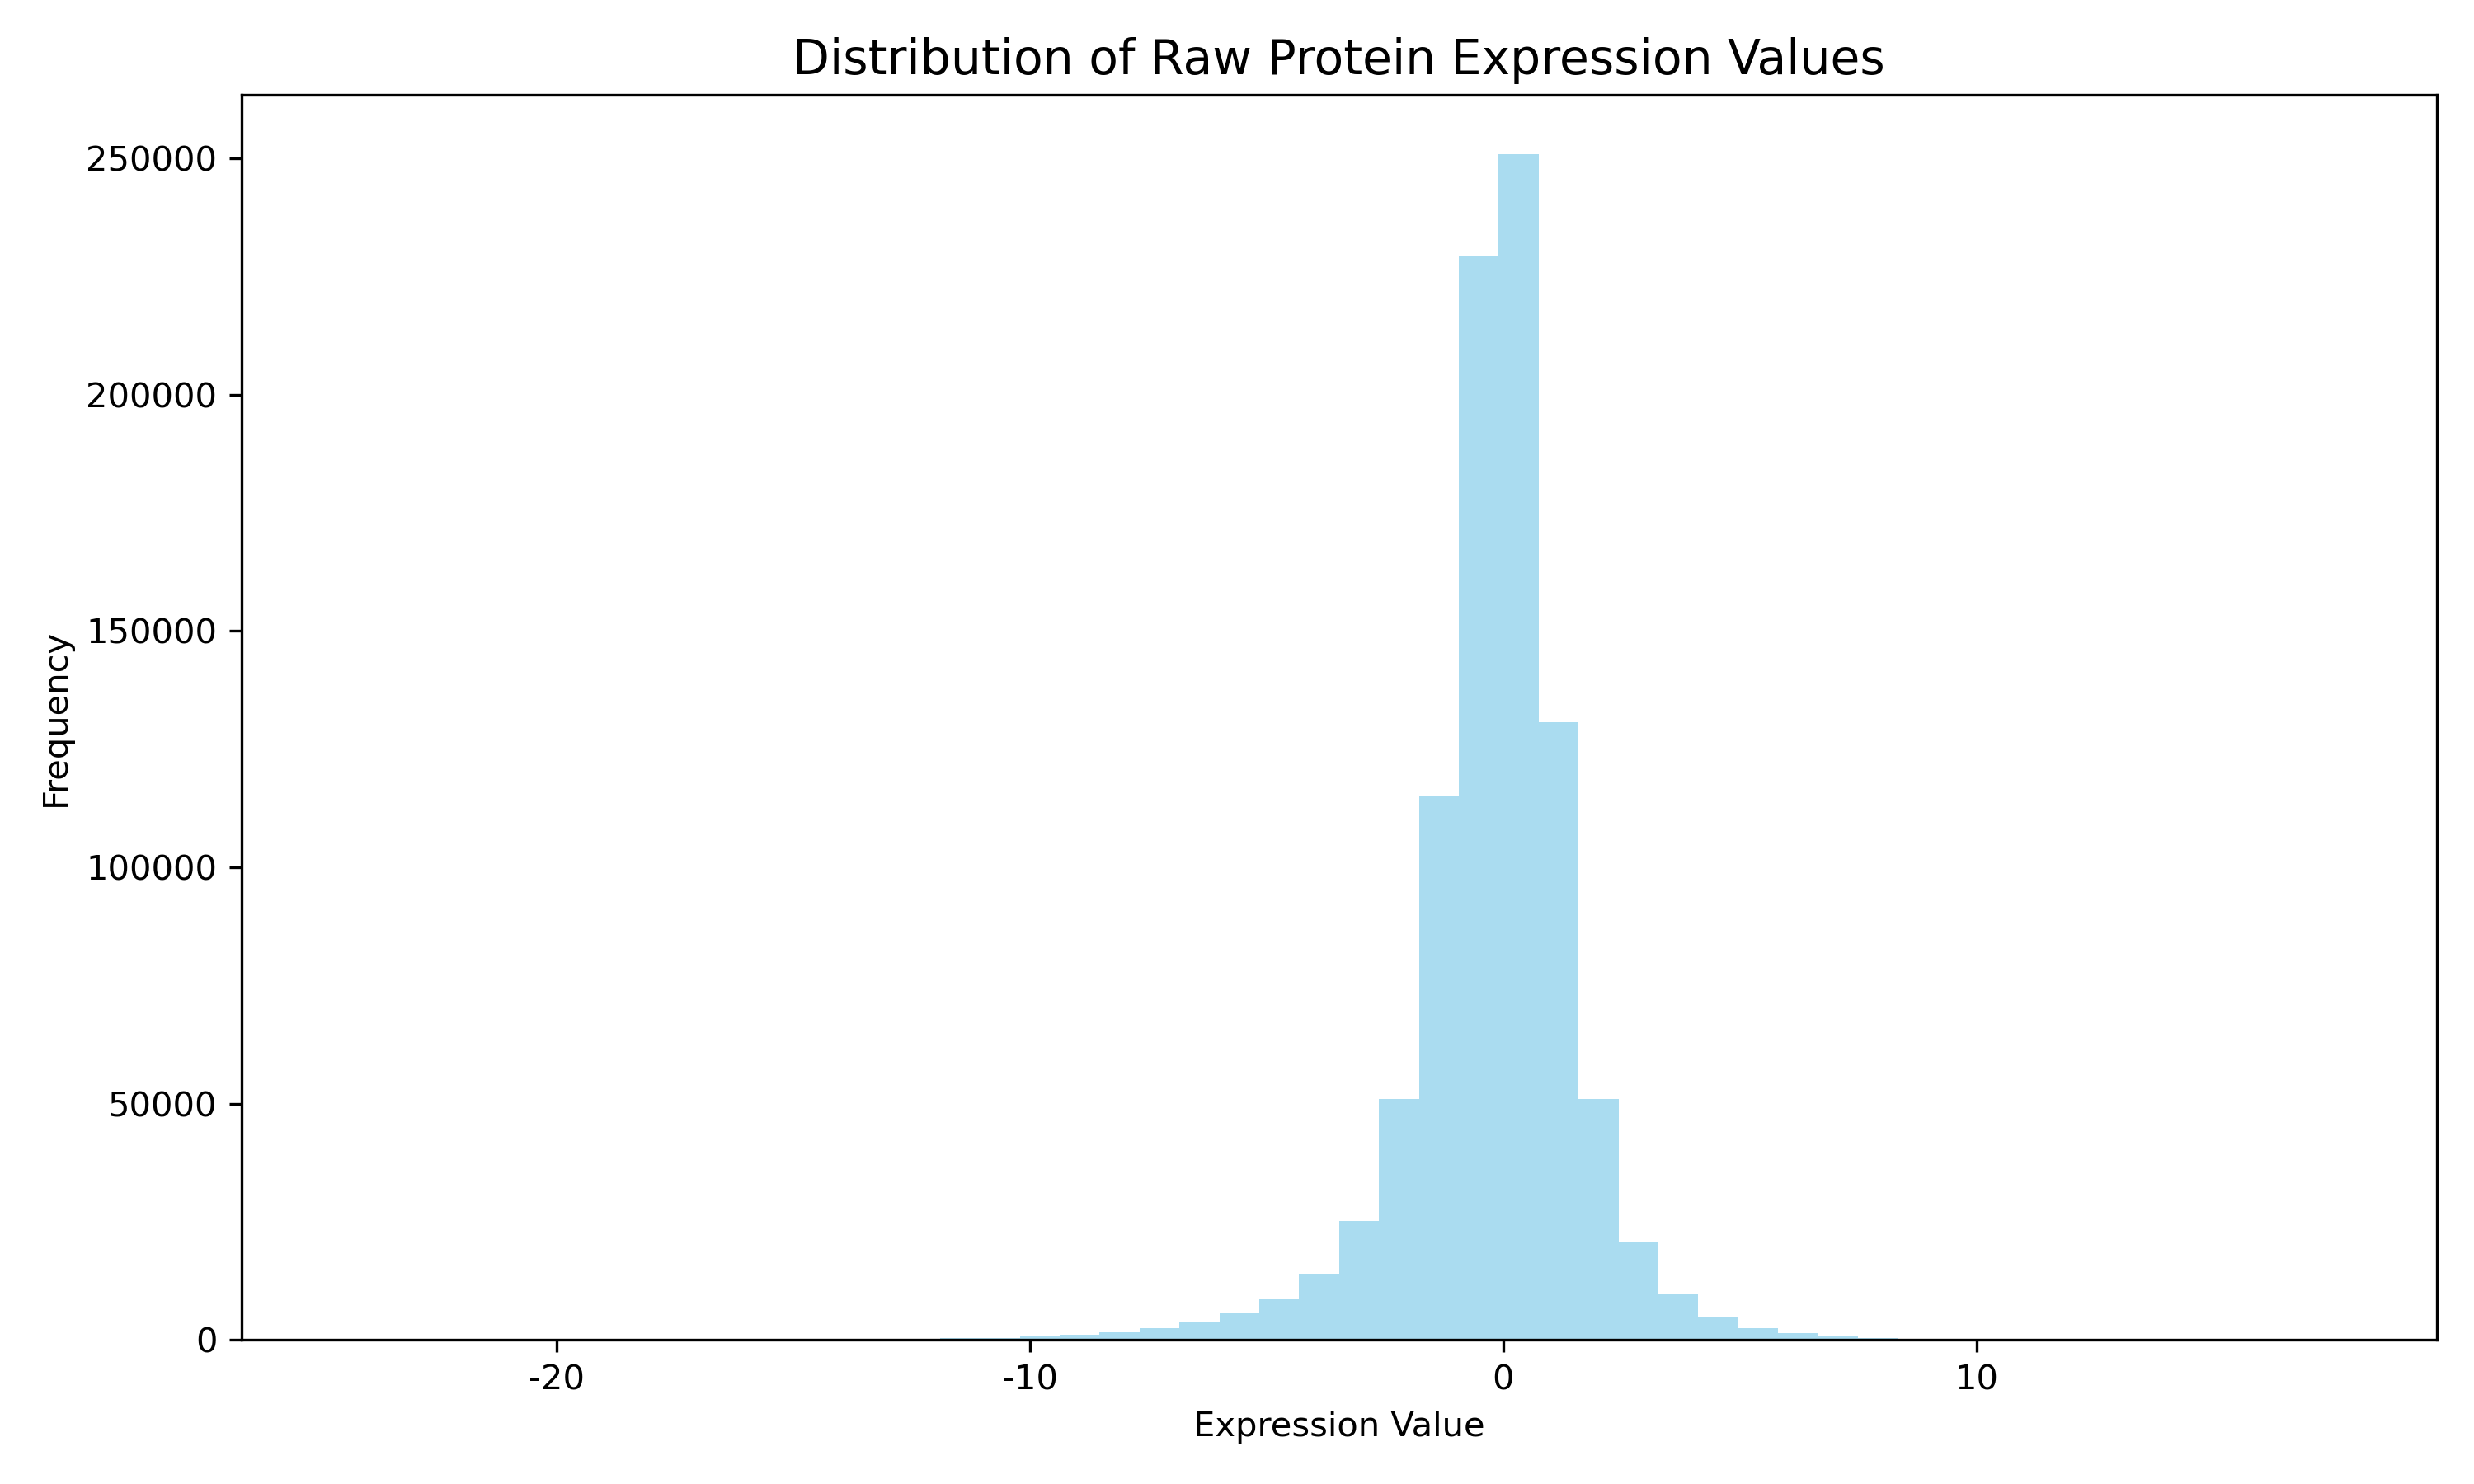
\includegraphics[width=0.85\textwidth]{./figures/data_preprocessing/2_distribution_raw_pro_value.png}
    \caption{原始蛋白质表达值直方图}
    \label{fig:raw_expr_dist}
\end{figure}
数据经过log2预处理后近似符合正态分布，无需额外分布转换操作。

\subsubsection{原始PAM50亚型分布}
\begin{figure}[htbp]
    \centering  
    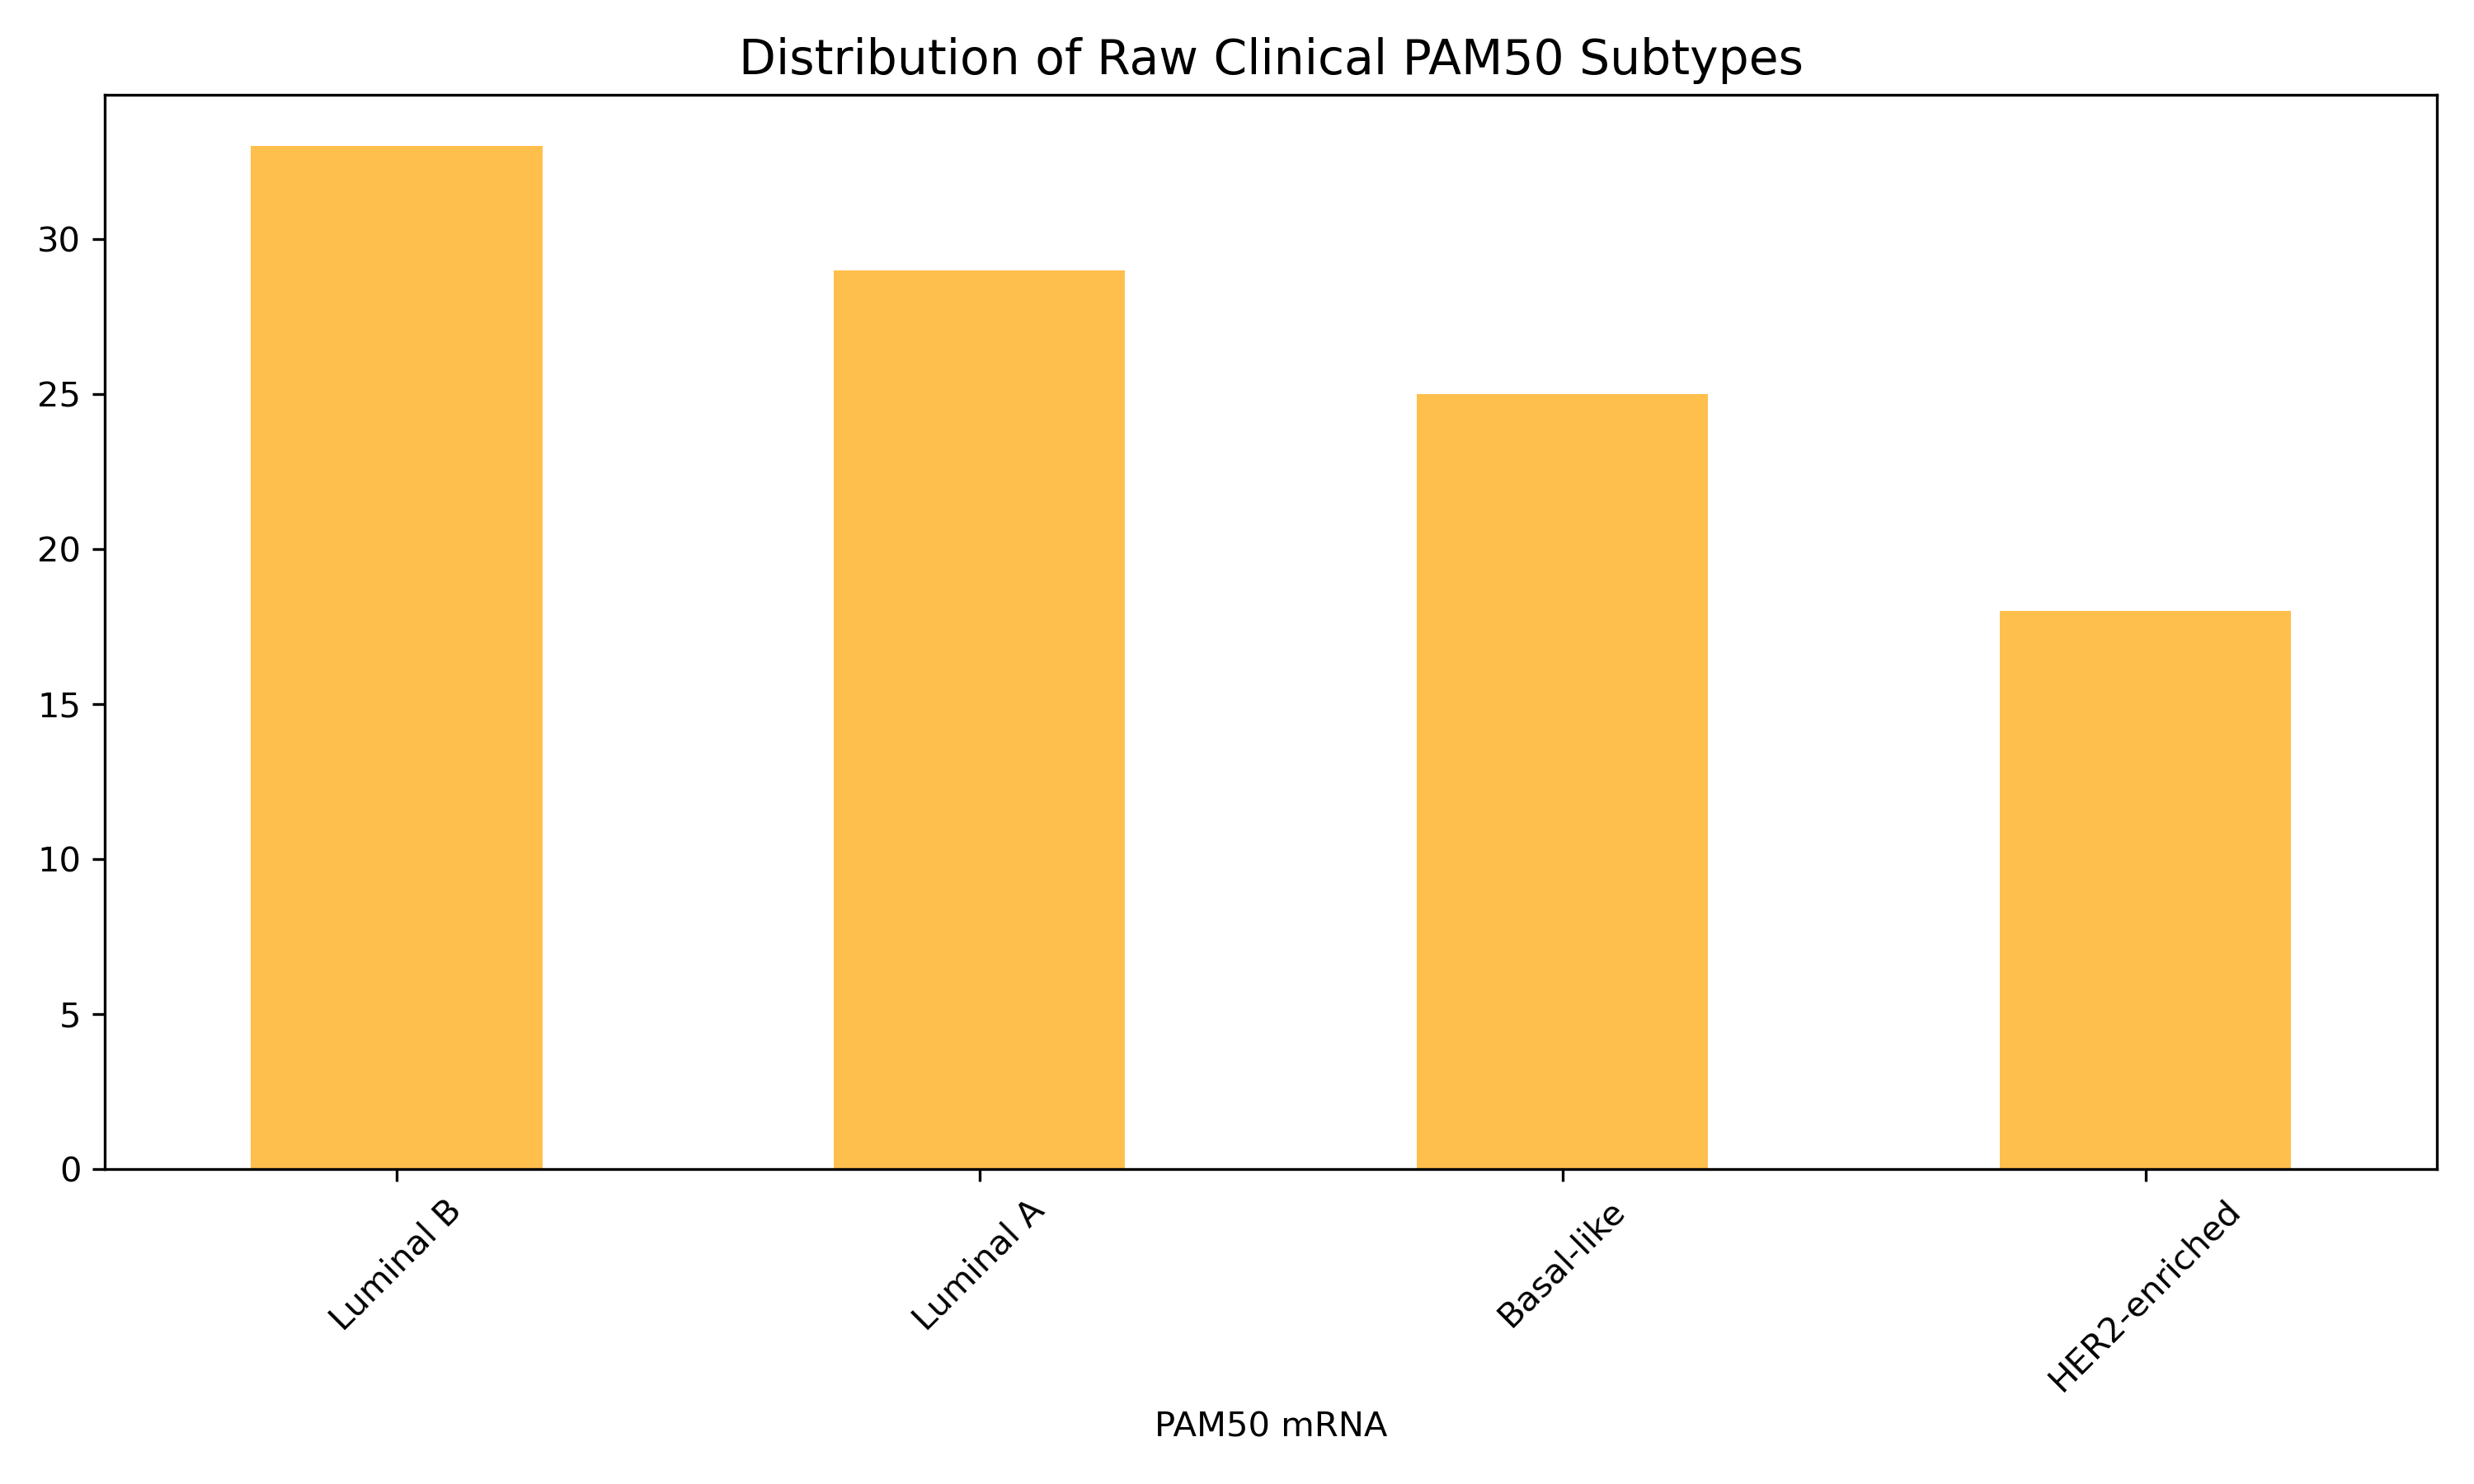
\includegraphics[width=0.85\textwidth]{./figures/data_preprocessing/3_distribution_raw_pam50.png}
    \caption{临床数据PAM50分子分型分布}
    \label{fig:raw_pam50_dist}
\end{figure}
临床数据中的 PAM50 标签存在一定类别差异，其中 Luminal B 亚型样本数量最高；在最终匹配到蛋白质组数据的 77 个样本中，各类别数量分别为 Luminal B 24 例、Luminal A 23 例、Basal-like 18 例和 HER2-enriched 12 例。

\subsubsection{处理后蛋白质表达值分布}
\begin{figure}[htbp]
    \centering
    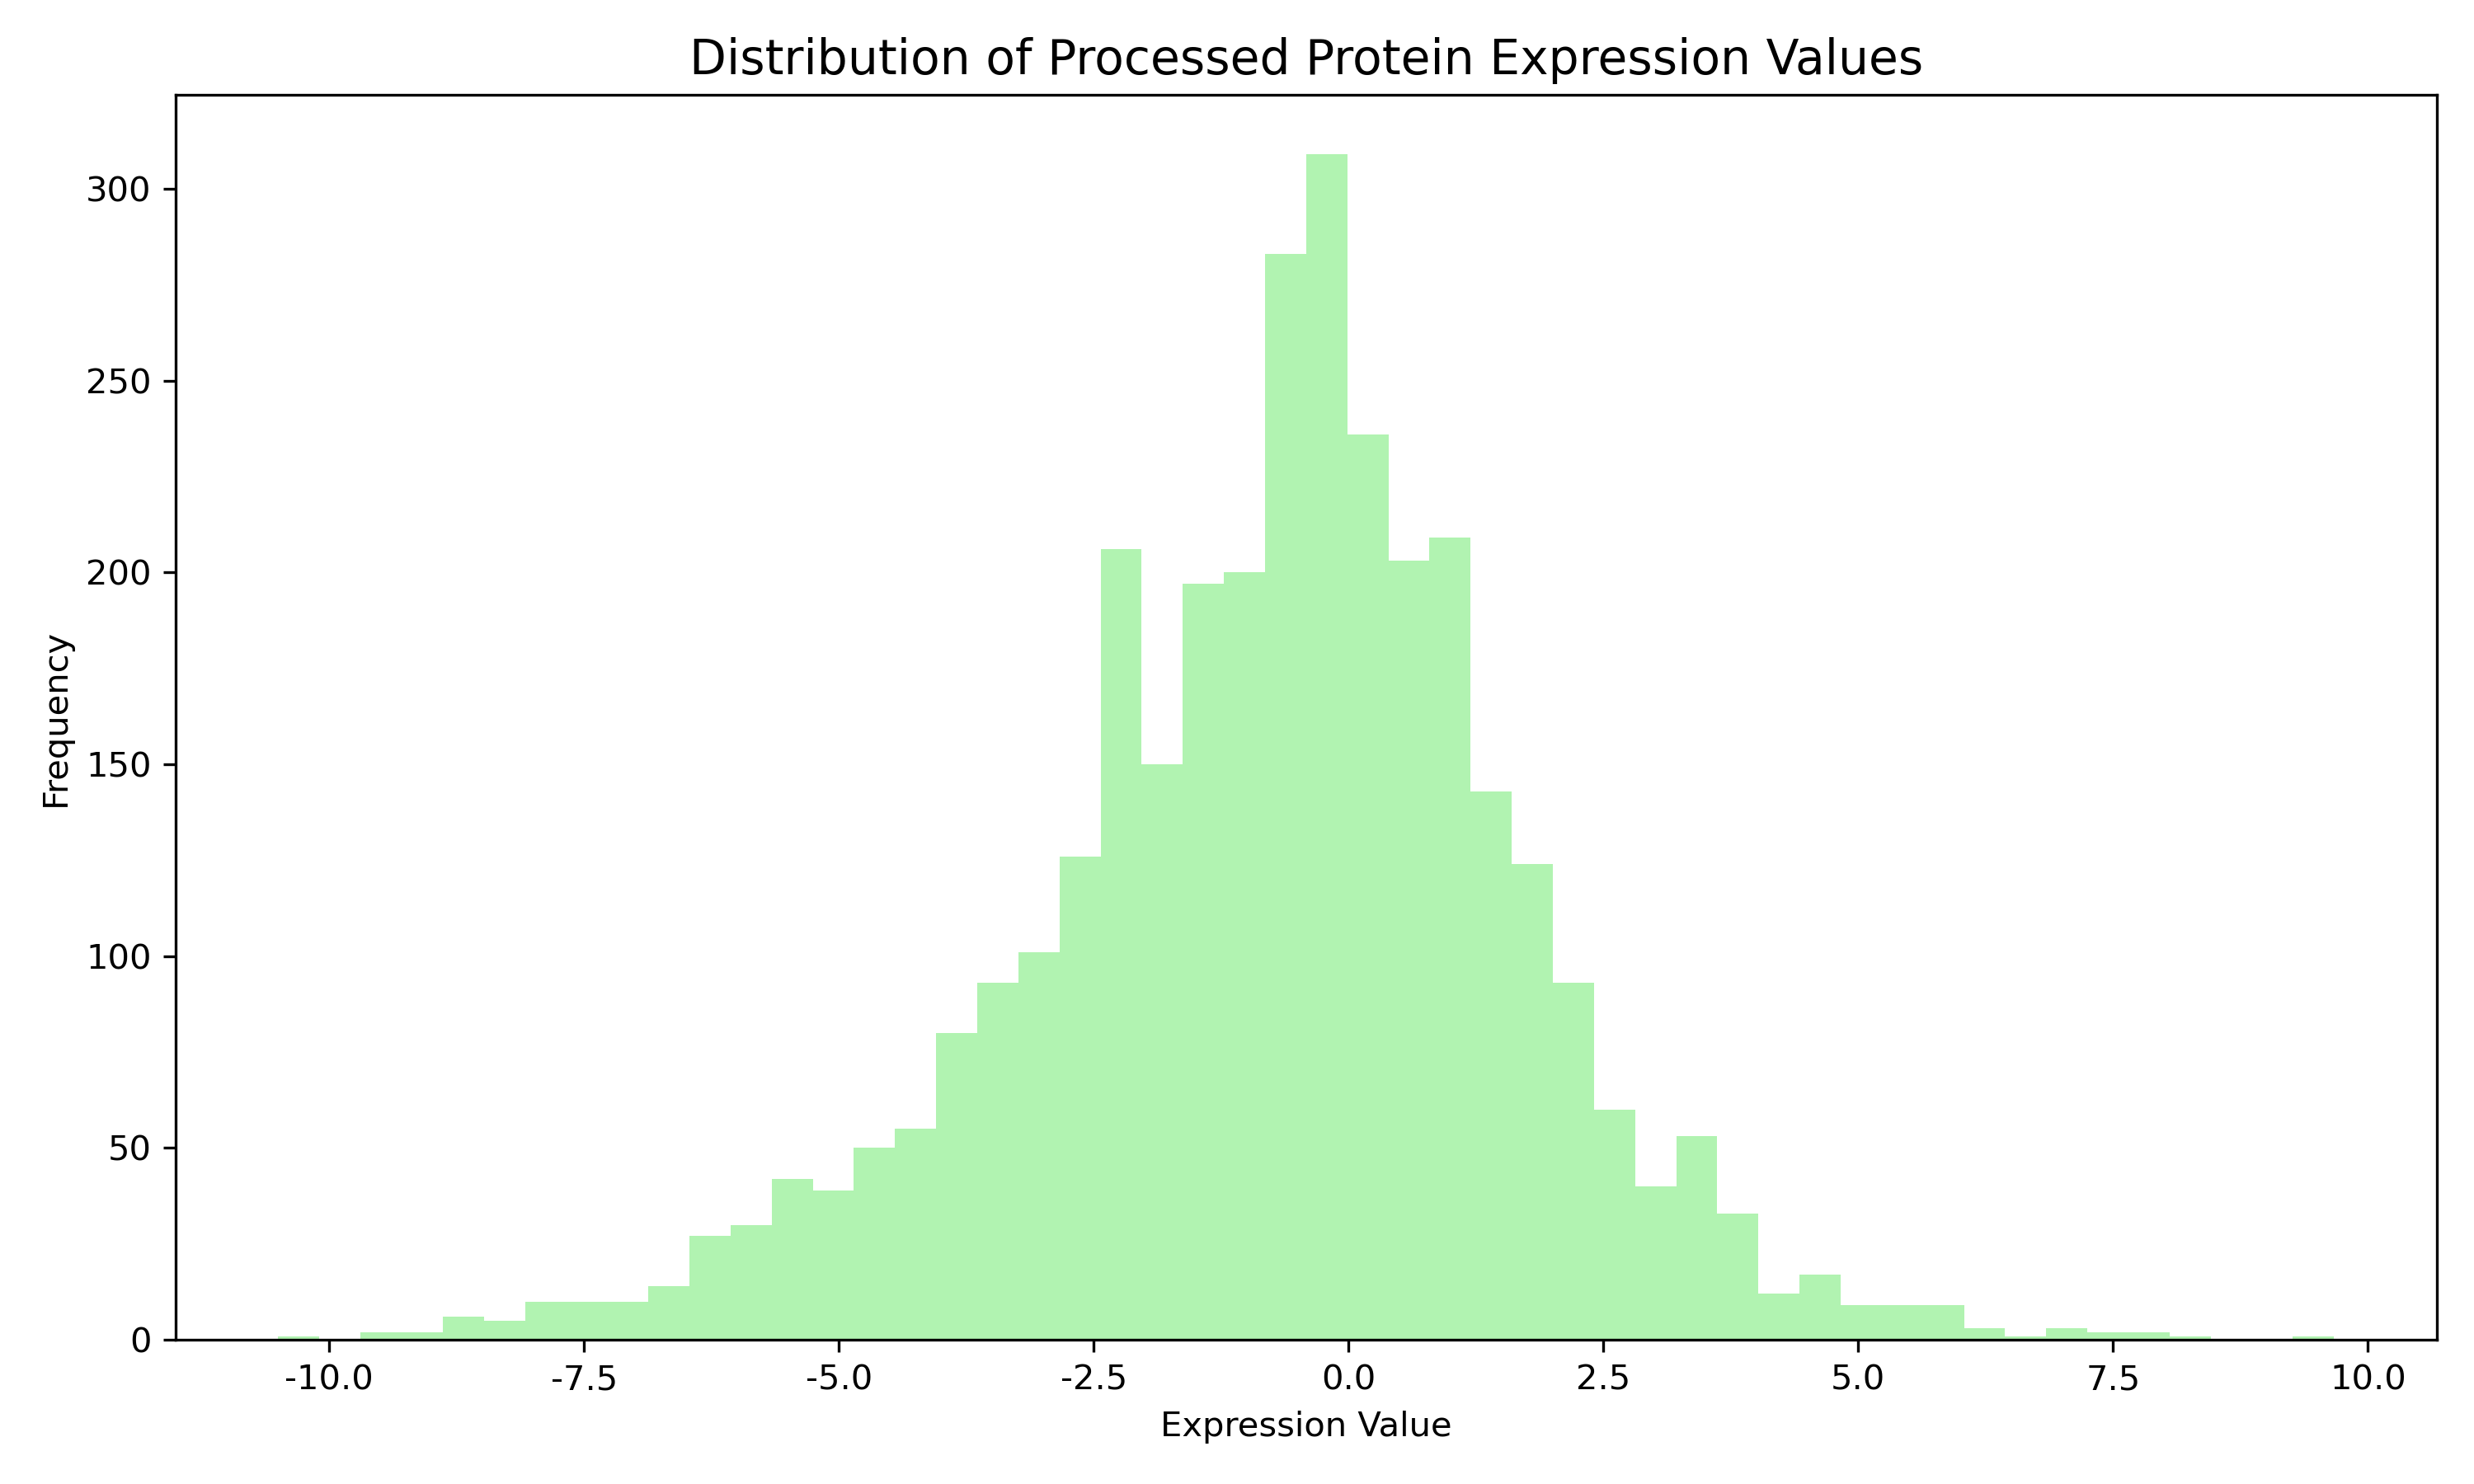
\includegraphics[width=0.85\textwidth]{./figures/data_preprocessing/4_distribution_processed_pro_value.png}
    \caption{缺失值填充后表达值分布}
    \label{fig:proc_expr_dist}
\end{figure}
填充前后数据形态连贯，整体分布未发生明显偏移，处理方式具备有效性。

\subsubsection{训练集与测试集PAM50分布对比}
\begin{figure}[htbp]
    \centering
    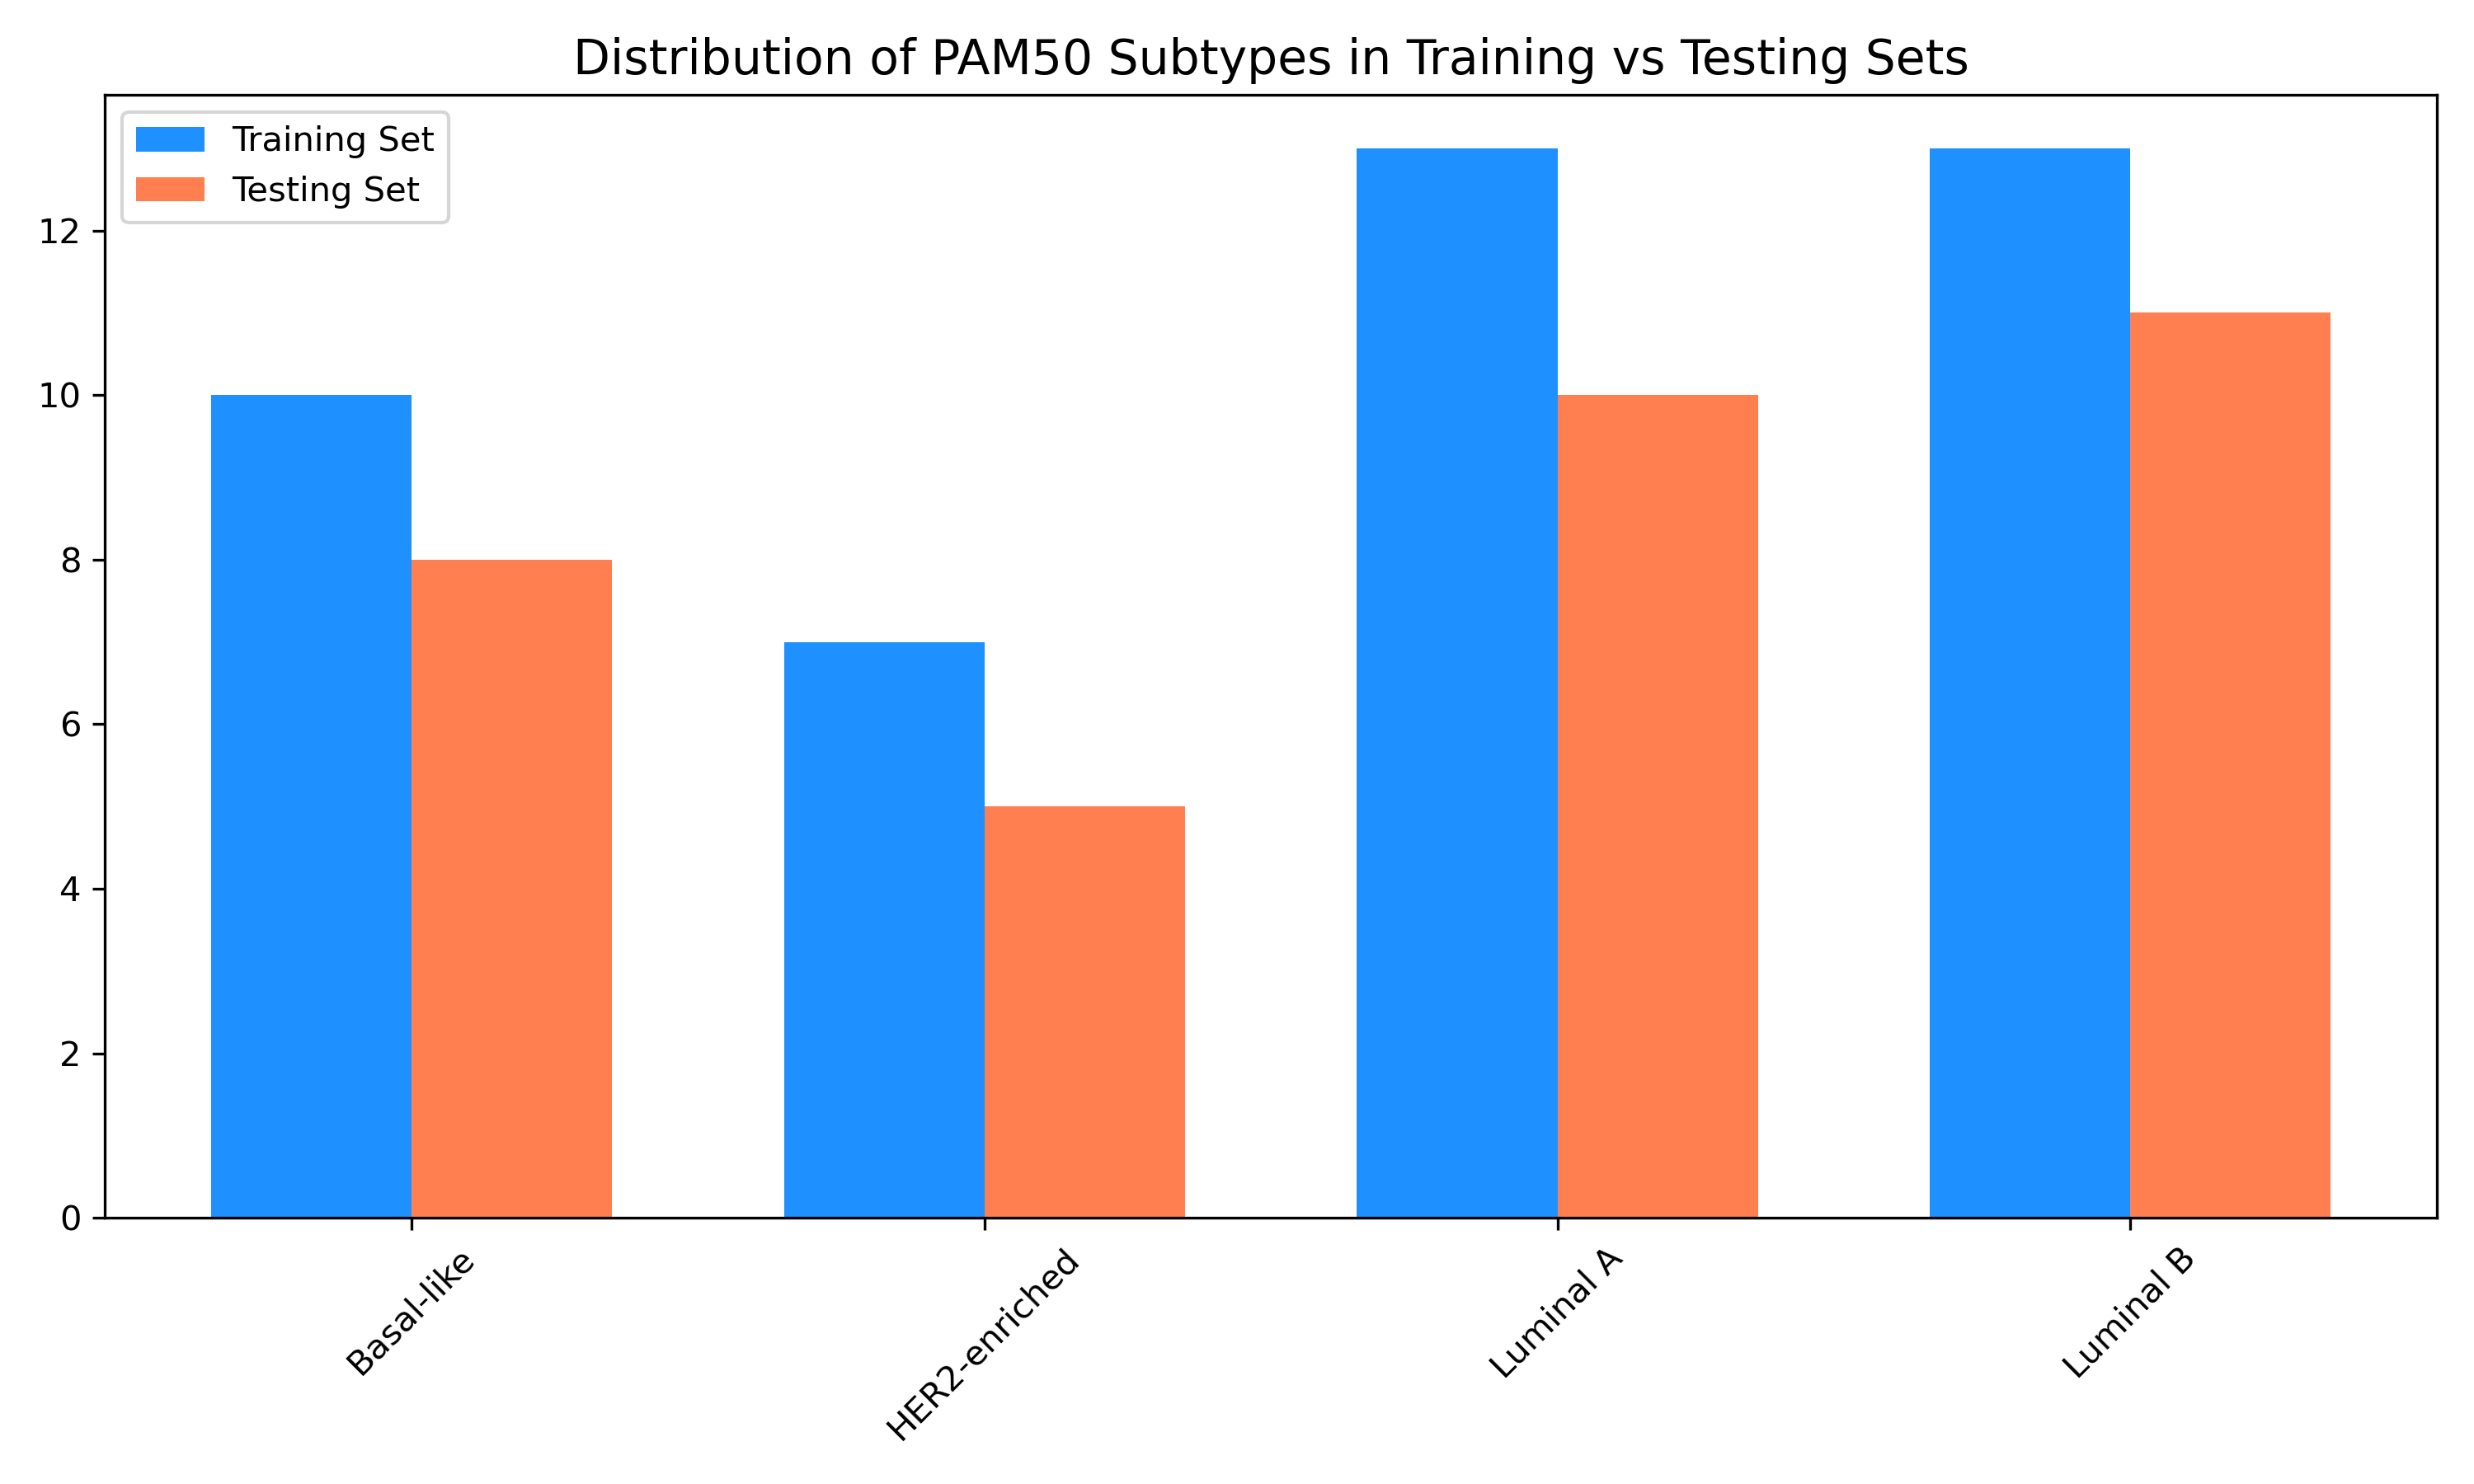
\includegraphics[width=0.85\textwidth]{./figures/data_preprocessing/5_training_testing_pam50_comparison.png}
    \caption{训练集与测试集PAM50亚型分布对比}
    \label{fig:train_test_pam}
\end{figure}
两组数据集亚型占比基本持平，分层抽样达到预期均衡效果。

\subsection{预处理统计汇总}
\begin{table}[htbp]
    \centering
    \caption{数据预处理各阶段统计信息}
    \begin{tabular}{lccc}
        \toprule
        处理阶段 & 样本数 & 特征数 & 处理方式 \\
        \midrule
        原始表达矩阵 & 83列 & 12553 & 含重复列与健康样本列 \\
        去重后表达矩阵 & 80列 & 12553 & 删除3个重复TCGA列 \\
        癌症样本匹配后 & 77例 & 12553 & 去除3个健康样本列并匹配临床ID \\
        PAM50特征筛选后 & 77例 & 43 & 与 \texttt{RefSeqProteinID} 匹配 \\
        训练集 & 43例 & 43 & 分层抽样，中位数填充后无缺失 \\
        测试集 & 34例 & 43 & 分层抽样，中位数填充后无缺失 \\
        \bottomrule
    \end{tabular}
\end{table}

\subsection{处理总结}
\begin{enumerate}
    \item 完成数据清洗、编号规整、矩阵结构调整等基础操作。
    \item 实现表达数据与临床标签精准匹配，筛选有效建模特征。
    \item 缺失值、异常值处理合理，数据整体分布保持稳定。
    \item 标准化消除量纲影响，分层划分保证数据集分布一致性。
    \item 预处理后数据质量达标，可开展后续聚类与分类建模实验。
\end{enumerate}
